\documentclass[12pt,twocolumn]{article}
\usepackage[utf8]{inputenc}
\usepackage[english]{babel}
\usepackage[table,xcdraw]{xcolor}
\usepackage{physics}
\usepackage{fancyhdr}
\usepackage{geometry}
\usepackage{natbib}
\usepackage{graphicx}
\usepackage{float}
\usepackage{wrapfig}
%\usepackage{caption}
\usepackage[justification=centering]{caption}
\usepackage{subcaption}
\usepackage{gensymb}
\usepackage[export]{adjustbox}
\usepackage{hyperref}
\geometry{margin = 20mm}
\usepackage{mathtools}
\usepackage{amsmath}
\usepackage{indentfirst}
\usepackage{xurl}
\usepackage{t1enc}
\usepackage{setspace}



\title{Simulating detectors with Geant4 3rd report}
\author{Scientific Modeling Computer Laboratory\\Bendegúz Borkovits T7UR9P\\Supervisor: Ákos Horváth}
\date{March 2022}


\begin{document}

\maketitle

\section{Introduction}
This document contains a summary about the continuation of my Geant4 project. Last time, through guides, I was able to create an example simulation that showcased a Cherenkov detector and then I presented the ways of gaining and showcasing the output data yielded by the simulation.

For the past two weeks, I have been working on the original aim of the project, that is to simulate the NEBULA detector. To that end, I acquired knowledge about the construction and properties of the earlier mentioned detector, as well as made an attempt at installing a tool called smsimulator that would have allowed me to immediately gain a complete simulation of NEBULA.

\section{The NEBULA detector}

NEBULA itself is a plastic scintillator array with a large volume that is used to simulate and measure fast neutron events at the 100-300 MeV range that are emitted at forward directions in processes such as nuclear breakup. \cite{nebula} NEBULA is part of the SAMURAI beam line at the RIKEN RI Beam Factory in Wako, Japan, a heavy-ion research facility where the world's largest superconducting ring cyclotron is located. \cite{RI}

NEBULA contains neutron detectors (NEUT), charge-particle veto detectors (VETO) and these are separated into several modules that are made up of plastic scintillators (BC-408) and photomultiplier tubes (PMT) that are connected to the ends of the scintillators by light guides. The modules themselves are organized into a two-layer detector wall. Altogether, the wall consists of 120 NEUT and 48 VETO modules of which 24 are in reserve. \cite{nebula}

\begin{figure}[H]
    \centering
    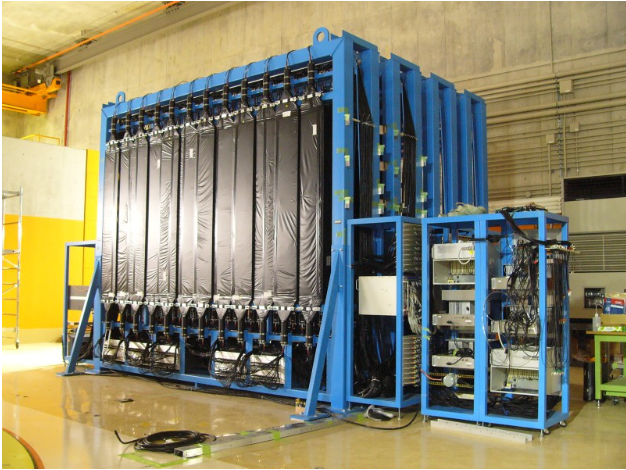
\includegraphics[scale = 0.65]{nebulakep.png}
    \caption{Showcasing the NEBULA detector at the RIKEN RI Beam Factory in Wako. \cite{nebula}}
\end{figure}

\section{Smsimulator and Geant4}

Smsimulator is a C++ program based on Geant4 that allows for the virtualization of NEBULA and is updated rather frequently. \cite{smsim} It offers a few services such as, simulating response to a single neutron, simulating trajectory of charged fragment in the SAMURAI magnet and a simulation for N-body neutron decay. The program uses ROOT libraries for visualisation. Due to these qualities, this simulation tool would be extremely useful. However, installing it is no easy feat as it requires numerous adjustments in the configuration files of ROOT and Geant4 and is also only compatible with a few specific versions of Geant4. Due to the earlier mentioned reasons, I have been unable to install and run smsimulator. After consulting with my supervisor, we opted to use the NEBULA simulation made by Balázs Pál, two years prior. \cite{masterdesky} However, after applying a few modifications and attempting to run said program, an error occurred that originates from the original simulation and thus needs more time to be resolved.

\section{Discussion}

Although the efforts made towards installing smsimulator have proven to be less than successful, I continue to work on the NEBULA simulation using Geant4. \cite{geant} After resolving the programming issue that has arisen, my first task will be to simulate the event of a neutron with 100 MeV colliding with the detector wall.

\bibliographystyle{plain}
\bibliography{references.bib}





\end{document}
